\documentclass{article}

\usepackage{times}
\usepackage{amssymb, amsmath, amsthm}
\usepackage[margin=1.5in]{geometry}
\usepackage{enumitem}
\usepackage{graphicx}
\usepackage{float}

\newenvironment{axioms}
 {\enumerate[label=\textbf{A\arabic*.}, ref=A\arabic*]}
 {\endenumerate}
\makeatletter
\newcommand\varitem[1]{\item[\textbf{A\arabic{enumi}\rlap{$#1$}.}]%
  \edef\@currentlabel{A\arabic{enumi}{$#1$}}}
\makeatother

\newtheorem{theorem}{Theorem}[section]
\newtheorem{corollary}{Corollary}[theorem]
\newtheorem{lemma}[theorem]{Lemma}

\begin{document}

\title{Projective Incidence Geometries and Models}
\author{Philip Warton}
\date{\today}
\maketitle


\section{Introduction}

Introduction needs to be rewritten entirely. \\

When talking about geometry, there are many rules, theorems, and axioms that one takes for granted. Because of this, one could assume that geometry as a whole is quite complex. In this sense, finite geometries are the minimalist geometries, where the rules are as simple as possible. This paper looks to explore the finite geometries, and find the more complex analogues of finite projective geometries such as Fano's projective plane. First, we will introduce finite geometries that we know and understand already, and introduce these to the reader to give a basis for understanding, and then go beyond this. \\\\
To go further means to first do some counting. Assume axioms, and generalize their theorems for $n$ points. We will start by doing this for axioms of the four-point geometry, and then ultimately make an attempt to do this for the Fano and Young plane geometries. There may be some experimentation with which axioms we choose to keep, remove, or alter in order to find generalized patterns. Once this process is complete we will present the results of the more complex projective geometries, and choose a particular one of these to examine. The goal is to then build a robust and elegant model for this geometry, that will then be presented to the reader.s

\subsection{Incidence Geometry}
It is important that we first answer the question: what is an incidence geometry? What does it mean for a geometry to be finite? In typical two-dimensional Euclidean geometry, we have two coordinates, $x$ and $y$, that determine a point. Our only restriction is that $x$ and $y$ must be real numbers (in modern interpretations of Euclidean geometry). Since there are infinitely many real numbers, by extension there are infinitely many Euclidean points. Since any two points determine a single line --- the straight line passing through both --- we say that there are infinitely many lines as well. \\

Before we continue, let us assume that something is a geometry if it relates points and lines in some capacity. So how would one construct a finite geometry? One might attempt to look at the Euclidean plane where points are restricted to the Cartesian product of $([0,1] \times [0,1])$. While we have certainly made a geometry that consists of a smaller infinity, it is certainly not finite as $[0,1]$ is a compact set with infinitely many distinct numbers. So let us make this more finite by taking only lattice points from this geometry, where $x,y \in \mathbb{Z}$. This leaves us with four points $a = (0,0), b = (0,1), c = (1,0)$, and $d=(1,1)$. Now we have a proper finite geometry. Let us ignore notions of distance and angle, and focus solely on the incidence of this geometry as in points, lines and their intersections. \\ 

Assume that the property of Euclidean geometry of 2 points determining a line still holds. Then, we know that there is a line through $(0,0)$ and $(0,1)$, another through $(0,0)$ and $(1,0)$, and so on for each combination of points, \fbox{Figure 1}.

\begin{figure}[h]
\centering
  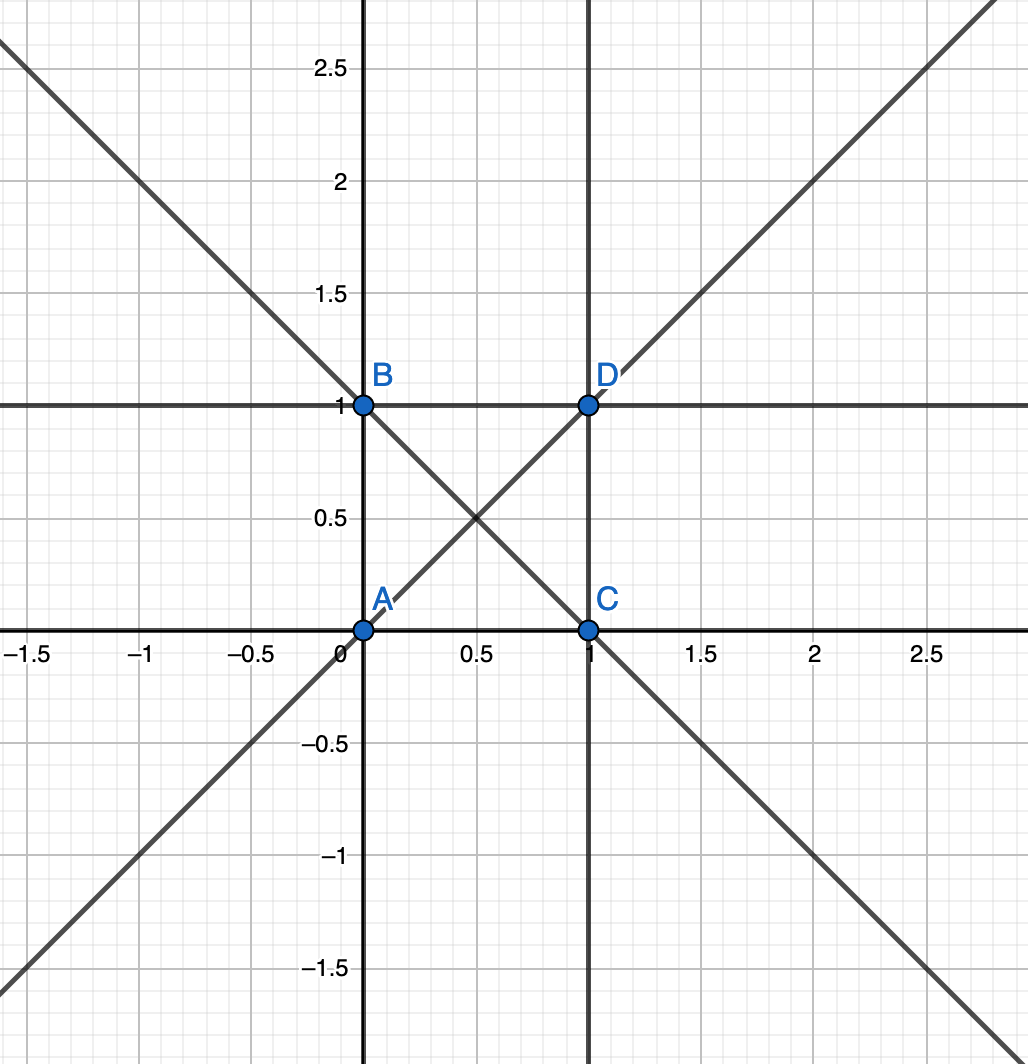
\includegraphics[scale=.3]{final_paper_plot_1}
  \caption{Finite Euclidean Geometry}
  \label{fig:boat1}
\end{figure}

The interesting results occure when we ask questions such as: Do $\overline{AD}$ and $\overline{BC}$ intersect? They certainly appear to intersect. However, we say that two lines if they meet at a point, i.e. if they share a point of intersection. By this definition, no such point exists, because we have not defined that point $(0.5,0.5)$ in our geometry. We say that two lines are parallel if they do not intersect, and by this definition the two crossing lines are parallel. This examination of exclusively the points and lines is at the core of finite geometries, and in fact, what we have described here is a model for the four point affine plane geometry.

\subsection{Examples}
\subsubsection{The Four Point Geometry}
See the section \fbox{Incidence}
\subsubsection{The Nine Point Affine Plane}
Maybe outside of the scope of this paper...
\subsection{Desired Results}
We wish to find an incidence geometry where there are no parallel lines. This quickly becomes difficult to model using the Euclidean plane and Euclidean lines. We begin to bend and stretch our lines to make the models fit the geometries they represent. While these ideas may seem bizzare, the underlying geometries are strong enough to extend to even more advancde structures, such as the real and complex projective planes. The intent of this paper, however, is to increase the complexity of the projective plane while remaining in the world of finite geometries. 

\section{Projective Planes}

\subsection{Duality}
\subsection{Degenerate Projective Planes}
Let us begin with the trivial cases, and if there are obvious patterns there perhaps they will extend to a generalized projective plane. We will omit the 0 point and 1 point projective planes, as their axioms and results will not be of great use.
\subsubsection{Order 2}
The two-point projective plane may exist, but if its axioms are similar to those of Fano's geometry, then it will be missing the key duality properties of projective geometry. Suppose we draw one line, with exactly two points. Then, we need

\subsection{Fano Plane}
State theorems (don't prove them), show model, discuss...
\subsection{The Order 4 Projective Plane}
\subsubsection{Axioms}
The axioms for the order four projective plane are as follows.
\begin{axioms}
  \item There exists a line.
  \item Every line has exactly four points.
  \item Not all points are on one line.
  \item Two points determine a single line.
  \item For every pair of lines, there exists a point that is on both.
\end{axioms}

The first theorem for us to prove is taken directly from what we know about the Fano Plane. The proof is identical as we only changed $\mathbf{A2}$, which this theorem is independent of.

\begin{theorem}
For every pair of lines there is exactly one point of intersection.
\end{theorem}

\begin{proof}
Suppose we have a pair of lines, $l_1, l_2$. By $\mathbf{A5}$, we have one point $p$ of intersection. By contradiction, suppose there was another distinct point $q$ that was on both $l_1$ and $l_2$. Then, the two points $p$ and $q$ determine $l_1$, and also $l_2$, which violates $\mathbf{A4}$.
\end{proof}

Our next theorem does not come quite as easily. In fact, developing this theorem requires that we construct and keep track of many points, lines and their intersection points. Although in Fano's plane, the analogous proof was readable in written paragraph form, I intend to introduce some new notation to our incidence geometries so that we can more easily understand the geometries we construct. \\

In previous proofs, it has been enough to simply state that points $p$ and $q$ lie on some line $l$, and to say that lines $l$ and $m$ intersect at some point $p$. However, it quickly becomes obvious that this can become quite convoluted as the number of points and lines increase. One must read through an entire paragraph in order to recall if a point $p$ lies on a particular line $l$. \\

It is for this reason that I intend to use a table of binary values where each column represents a point, and each row represents a line. Then to check if point $p$ lies on line $l$, refer to row $l$ column $p$ and verify that a 1 is written there. We can look at the four point affine plane in this way, \fbox{Figure Something}.

\begin{center}
\begin{tabular}{ c|c|c|c|c } 
 
  & $p_1$ & $p_2$ & $p_3$ &$p_4$\\ 
\hline
 $l_1$ & 1 & 1 & 0 & 0\\
 \hline
 $l_2$ & 1 & 0 & 1 & 0\\
 \hline
 $l_3$ & 1 & 0 & 0 & 1\\
 \hline
 $l_4$ & 0 & 1 & 1 & 0\\
  \hline
 $l_5$ & 0 & 1 & 0 & 1\\
 \hline
 $l_6$ & 0 & 0 & 1 & 1\\
\end{tabular}
\end{center}

Though it may not be immediately obvious, this model will be useful for checking certain conditions. As you may remember, when drawing the four point affine plane, there were two lines that appeared to cross but did not intersect. With this model, no such comprimise must be made. Should you look at two lines $l_3$ and $l_4$, it is clear if they share a point or not.
\begin{center}
\begin{tabular}{ c|c|c|c|c } 
 
  & $p_1$ & $p_2$ & $p_3$ &$p_4$\\ 
 \hline
 $l_3$ & 1 & 0 & 0 & 1\\
 \hline
 $l_4$ & 0 & 1 & 1 & 0\\
\end{tabular}
\end{center}
 In this case $l_3$ and $l_4$ are parallel. \\
 
 With this in mind, we introduce the next, and seemingly most important, theorem.
 \begin{theorem}
 There are exactly 13 points and 13 lines.
 \end{theorem}
 
 \begin{proof}
 By $\mathbf{A1}$, there exists a line $l_1$, and by $\mathbf{A2}$, there are exactly four points on this line, which we will call $p_1, p_2, p_3, p_4$. Because of $\mathbf{A5}$, there must exist an additional point $p_5$ that is not on $l_1$. Then, $p_5$ and $p_1$ must determine a new line $l_2$. Otherwise, $p_5$ would lie on $l_1$ and $\mathbf{A2}$ would be violated. 
 \begin{center}
\begin{tabular}{ c|c|c|c|c|c } 
 
  & $p_1$ & $p_2$ & $p_3$ &$p_4$ &$p_5$\\ 
 \hline
 $l_1$ & 1 & 1 & 1 & 1 & 0\\
 \hline
 $l_2$ & 1 & 0 & 0 & 0& 1\\
\end{tabular}
\end{center}
We must construct additional points $p_6, p_7$ that lie on $l_2$, so that $l_2$ has four points on it. If we choose any of our previous points, then $l_1$ and $l_2$ would have more than one point of intersection, violating \fbox{Theorem 2.2}. Similarly, there must be a line determined by $p_5$ and $p_2$ that is not $l_1$ or $l_2$, since if $p_1$ and $p_2$ both were on a line other than $l_1$, $\mathbf{A4}$ would be violated. We will call this new line $l_3$. We must construct two more points $p_8, p_9$ that lie on $l_3$. Then, $l_4$ consists of points $p_3, p_5, p_{10}, p_{11}$, and finally $l_5$ contains $p_4, p_5, p_{12}, p_{13}$. At this point, let us omit zeroes from our incidence tables for visual clarity.
\begin{center}
\begin{tabular}{ c|c|c|c|c|c|c|c|c|c|c|c|c|c } 
 
  & $p_1$ & $p_2$ & $p_3$ &$p_4$ &$p_5$ &$p_6$ &$p_7$ &$p_8$ &$p_9$  &$p_{10}$&$p_{11}$&$p_{12}$&$p_{13}$ \\ 
\hline
 $l_1$ & 1 & 1 & 1 & 1 &  &&& &&&&& \\ 
 \hline
 $l_2$ & 1 & &&&1&1&1&&&&&& \\
 \hline
 $l_3$ & &1&&&1&&&1&1&&&&\\
 \hline
 $l_4$ &  &  & 1 &  &1 & &&&&1&1&&\\
 \hline
 $l_5$ & &&&1&1&&&&&&&1&1\\


\end{tabular}
\end{center}
We now have the existence of 13 points. We will return to the number of points --- and showing that there are only 13 --- after we have shown the existence of 13 lines. \\

So far we have shown the existence of 5 lines. What we have so far is not complete. By $\mathbf{A4}$, $p_1$ and $p_8$ must determine a single line. This must be a new line $l_6$, otherwise we would need to say that one of our current lines is incident with another point, which would cause there to be 5 points on one line, violating $\mathbf{A2}$. Similarly, another line will be determined by $p_1$ and $p_9$. Since $p_8$ and $p_9$ determine the line $l_3$, if $p_1$, $p_8$, and $p_9$ were co-linear then $p_8, p_9$ would determine $l_3$ and $l_6$, therefore there is a new line $l_7$ determined by $p_1$ and $p_2$.

\begin{center}
\begin{tabular}{ c|c|c|c|c|c|c|c|c|c|c|c|c|c } 
  & $p_1$ & $p_2$ & $p_3$ &$p_4$ &$p_5$ &$p_6$ &$p_7$ &$p_8$ &$p_9$  &$p_{10}$&$p_{11}$&$p_{12}$&$p_{13}$ \\ 
\hline
 $l_1$ & 1 & 1 & 1 & 1 &  &&& &&&&& \\ 
 \hline
 $l_2$ & 1 & &&&1&1&1&&&&&& \\
 \hline
 $l_3$ & &1&&&1&&&1&1&&&&\\
 \hline
 $l_4$ &  &  & 1 &  &1 & &&&&1&1&&\\
 \hline
 $l_5$ & &&&1&1&&&&&&&1&1\\
 \hline
 $l_6$ &1&&&&&&&1&?&?&?&?&? \\
 \hline
 $l_7$ &1&&&&&&&&1&?&?&?&?\\
 \end{tabular}
 \end{center}

Proof will be completed in final draft. We eventually come to the following result.

\begin{center}
\begin{tabular}{ c|c|c|c|c|c|c|c|c|c|c|c|c|c } 
 
  & $p_1$ & $p_2$ & $p_3$ &$p_4$ &$p_5$ &$p_6$ &$p_7$ &$p_8$ &$p_9$  &$p_{10}$&$p_{11}$&$p_{12}$&$p_{13}$ \\ 
\hline
 $l_1$ & 1 & 1 & 1 & 1 &  &&& &&&&& \\ 
 \hline
 $l_2$ & 1 & &&&1&1&1&&&&&& \\
 \hline
 $l_3$ & &1&&&1&&&1&1&&&&\\
 \hline
 $l_4$ &  &  & 1 &  &1 & &&&&1&1&&\\
 \hline
 $l_5$ & &&&1&1&&&&&&&1&1\\
 \hline
 $l_6$ &1&&&&&&&1&&1&&1& \\
 \hline
 $l_7$ &1&&&&&&&&1&&1&&1\\
 \hline
 $l_8$ &&1&&&&1&&&&1&&&1\\
 \hline
 $l_9$ &&1&&&&&1&&&&1&1&\\
 \hline
 $l_{10}$ &&&1&&&1&&&1&&&1&\\
 \hline
 $l_{11}$ &&&1&&&&1&1&&&&&1\\
 \hline
 $l_{12}$&&&&1&&1&&1&&&1&&\\
 \hline
 $l_{13}$ &&&&1&&&1&&1&1&&& 

\end{tabular}
\end{center}

We now have the existence of 13 points and 13 lines. Suppose there is a 14\textsuperscript{th} point $p_{14}$. Since all lines already have exactly four points, $p_{14}$ would have to be on some line $l_{14}$. This line must intersect all other lines by $\mathbf{A5}$. However, since all pairs of points in $\{p_1,p_2, \dots , p_{13}\}$ already determine one line, there is guarenteed to be a violation of axiom $\mathbf{A4}$. \\

Now suppose that there is a 14\textsuperscript{th} line. 

 \end{proof}
\subsection{Further Generalizations}

Once again perhaps outside the scope of this paper...\\

Finding Order 5 Projective plane may be plausible, but probably not a dot and line model for it, and probably not a rigorous proof for it either.

\section{Building a Model}
WIP... 

\subsection{Different Possible Models}
\subsection{The Final Most Elegant Model}

\section{Generalize $\dots$ ?}

\section{Conclusion}
As we have now looked at our model for the order four projective plane, we can think about what this may be used for. One application of this projective plane is (insert piece about group theory, symmetry, combinatorics, graphs, or cycles) (WIP)

\end{document}